\section{QM/MM Embedding}

\emph{Please continue to consider this functionality
  experimental and contact the maintainers before using it.}

When simulating nanostructured surfaces, it may be favorable to 
avoid the standard supercell approach and rather make use of a QM/MM
embedding approach. E.g. with clusters or molecules adsorbed, extensive 
supercells are required to avoid spurious interaction between the 
nanostructure and its periodic copies. This makes computations tedious.

In the QM/MM approach, one embeds a quantum mechanical (QM) region in an extended 
monopole field. To avoid spurious charge leakage out of the QM region positively 
charged monopoles in the vicinity are replaced by norm-conserving pseudopotentials
\cite{KleinmanBylander}. Those pseudopotential files can be either generated manually with 
the open source program package FHI98PP \cite{FuchsFHI98PP} or downloaded from \url{http://www.abinit.org/downloads/psp-links/lda_fhi} or
\url{http://www.abinit.org/downloads/psp-links/gga_fhi}. 

\begin{figure}[hb]
  \centering
  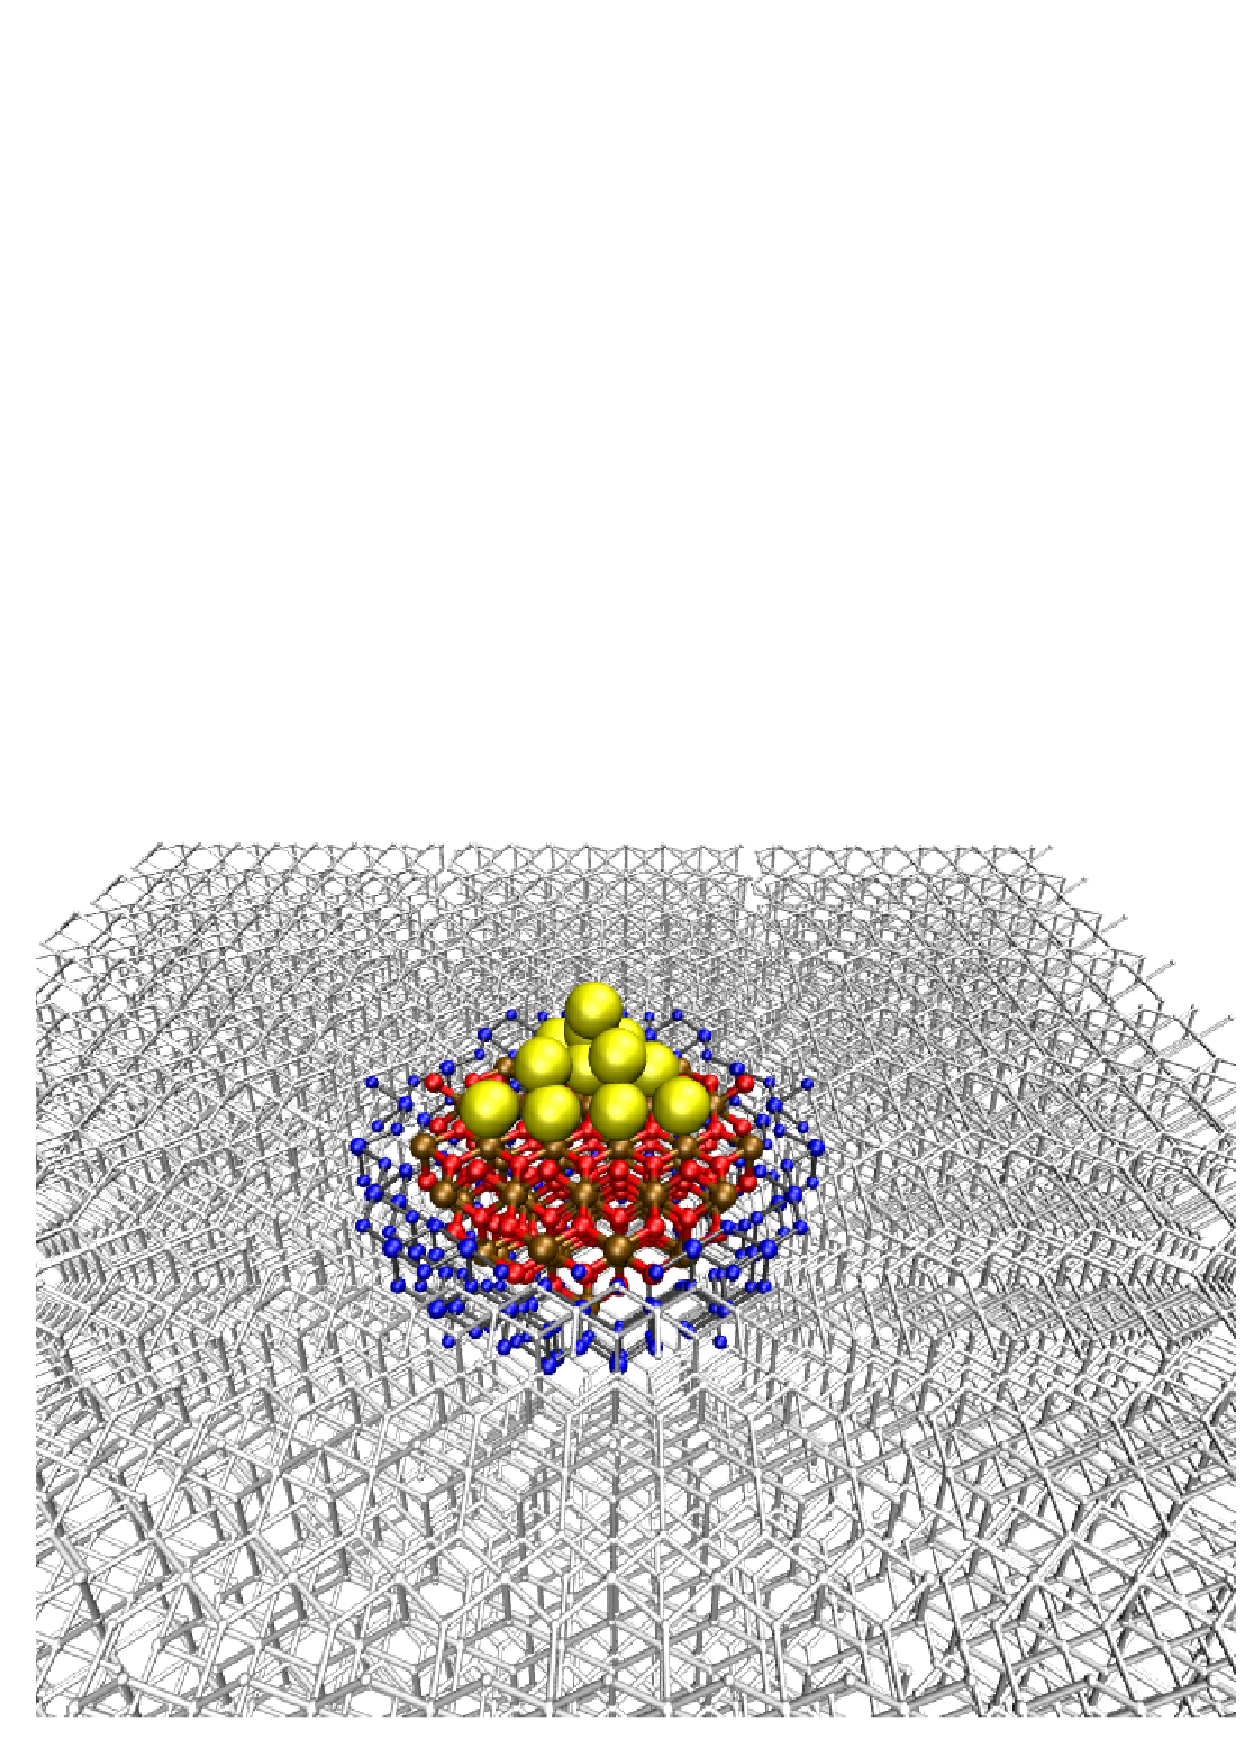
\includegraphics[width=0.7\textwidth]{qmmm}
  \caption{Example for QM/MM setup: $Au_n@TiO_2$. The adsorbed cluster and direct substrate vicinity defines the QM-region.
The far field surrounding (grey particles) pictures a monopole field with formal charges (4+ for Ti and 2- for O). In the blue 
region, oxygen particles are still represented as monopoles, however Ti-cations are described with ionic pseudopotentials.}
  \label{fig:qmmm_embedding}
\end{figure}

 
The QM/MM approach has the huge advantage ultimately also being capable to efficiently 
deal with \textbf{charged} systems, which will be a fundamental asset for the 
description of surface electrochemistry or photo-induced catalysis.


\emph{QM/MM embedding is not applicable for metal substrates for physical reasons.}



% \emph{This functionality is not yet available for periodic systems.}

\newpage

\subsection*{Tags for \texttt{geometry.in}:}


\keydefinition{pseudocore}{geometry.in}
{
  \noindent
  Usage: \keyword{pseudocore} \option{x} \option{y} \option{z}
    \option{species} \\[1.0ex] 
  Purpose: Places the center of a pseudopotential at a
    specified location. \\[1.0ex]
  \option{x} : $x$ coordinate of the pseudocore. \\
  \option{y} : $y$ coordinate of the pseudocore. \\
  \option{z} : $z$ coordinate of the pseudocore. \\
  \option{species} : string defining the name of the pseudoized species; this needs to correspond to name specified in control.in . \\
}

The keyword \keyword{pseudocore} should be used for those particles
replaced by pseudopotentials, so cations. Anions are to be treated simply
as monopoles, employing the \keyword{multipole} infrastructure.

% \vspace{2cm}
% \begin{center}
% !!! At one point I should add a script for constructing a divided surface!!!\end{center}
% 
% \newpage

\subsection*{Tags for general section of \texttt{control.in}:}

Only species data concerning the pseudoized species mentioned in \texttt{geometry.in} 
need to be appended in the \texttt{control.in}.
Accept for some mandatory changes (listed below) those species data are essentially the same 
as you can find them in the species\_default folder. E.g. if you want to pseudoize for example titanium, 
take the $Ti$ default file as a template. However, \textbf{the pseudoized species must not have any basis functions 
accept for the minimal basis}. The minimal basis in needed to construct the integration weights, however in order 
to exclude the minimal basis from the actual quantum chemical calculation, the flag 
\subkeyword{species}{include\_min\_basis} needs to be set to \texttt{.false.}.


Although nomenclature is misleading as it is chosen at the moment, you do NOT need the \keyword{qmmm}
in order to make QM/MM embedding work. 




\begin{figure}[hb]
  \small
  \begin{verbatim}


[...]
  species        Ti_pseudo
#     global species definitions
    nucleus             22
    mass                47.867

    pseudo              Ti.cpi
    pp_charge           4.
    pp_local_component     1
    nonlinear_core      .false.

    include_min_basis .false.


[...]

  \end{verbatim}
  \normalsize

  \vspace*{-4.0ex}

  \caption{\label{Fig:control.in_qmmm}
Species data for a pseudoized titanium atom. Starting from the default species files 
only a few flags need to be added and the basis functions (accept the minimal basis) 
need to be removed.
  }
\end{figure}


Similar to all-electron \subkeyword{species}{atom}, FHI-aims expects all atom specifications  
like \subkeyword{species}{mass}, \subkeyword{species}{nucleus}, information for the integration grid etc.
Some additional flags need to be set that FHI-aims is able to realize them as pseudoized species.  

\subkeydefinition{species}{pseudo}{control.in}
{
  \noindent
  Usage: \subkeyword{species}{pseudo} \option{string} \\[1.0ex]
  Purpose: Parses the name of file the Kleinman-Bylander pseudopotential 
is written in \\[1.0ex]
  \option{string} name of file\\
}

FHI-aims expects the pseudopotential file to be in a specific formatting, namely the 
output format *.cpi of the generator program FHI98PP \cite{FuchsFHI98PP}.
FHI98PP expects this file to be in the same folder as control.in and geometry.in.

\subkeydefinition{species}{pp\_charge}{control.in}
{
   \noindent
   Usage: \subkeyword{species}{pp\_charge} \option{value} \\[1.0ex]
   Purpose: Specifies the charge of the pseudoized ion. \\[1.0ex]
   \option{value:} any real value is allowed\\
 }

 \subkeyword{species}{pp\_charge} must be the charge which has been
 set in the generation of the pseudopotential and equals the number of
 pseudoized valence electrons.  This parameter is needed for the far
 field extrapolation of the pseudopotential.


\subkeydefinition{species}{pp\_local\_component}{control.in}
{
  \noindent
  Usage: \subkeyword{species}{pp\_local\_component} \option{value} \\[1.0ex]
  Purpose: Specifies which l-channel of the pseudopotential should act as the local component.
Find a detailed theoretical background in \cite{FuchsFHI98PP}. \\[1.0ex]
  \option{value:} integer value\\
}

The choice which l-channel should be the local component is essential for the performance 
of the pseudopotentials. Again, read \cite{FuchsFHI98PP} for further help.


\subkeydefinition{species}{ nonlinear\_core}{control.in}
{
  \noindent
  Usage: \subkeyword{species}{ nonlinear\_core} \option{flag} \\[1.0ex]
  Purpose: when .true. FHI-aims expects and reads in a partial core density (and partial core density gradient)
 from the pseudopotential input file to take account of nonlocal core correction \cite{Louie1982}. \\[1.0ex]
  \option{flag} is a logical expression, either .true. or .false. Default: .false.\\
}

